\section*{Introduction}
La transcription automatique de la musique (TAM) est un défi ancien
\cite{first_one} et difficile qui n’est toujours pas résolu de manière
satisfaisante par les systèmes actuels. Il a engendré une
grande variété de sous-tâches qui ont donné naissance au domaine de la
recherche d’informations musicales (RIM)\footnote{\url{https://ismir.net/}}.
Actuellement, en raison de la nature séquentielle et symbolique des données
musicales et du fait que les travaux en TAL sont assez avancés en analyse de
données séquentielles ainsi qu’en traitement du signal, de nombreux travaux en
RIM font appel au TAL. Certains de ces travaux se concentrent notamment sur
l’analyse des paroles de chansons\footnote{NLP4MuSA, the 2nd Workshop on
Natural Language Processing for Music and Spoken Audio, co-located with ISMIR
2021.}.

Dans ce chapitre, nous traiterons de l’informatique musicale, nous montrerons
les liens existants entre la RIM et le TAL ainsi qu’entre les notions de
langage musical et de langues naturelles. Nous traiterons également du problème
de la TAM et de ses applications. Enfin, nous décrirons les représentations de
la musique qui sont nécessaires à la compréhension du présent travail.

\section{Informatique musicale et langues naturelles}
L’informatique musicale ou \textit{Computer Music} regroupe l’ensemble des
méthodes permettant de créer ou d’analyser des données musicales à l’aide
d’outils informatiques \cite{book_muller}. Ce domaine implique l’utilisation de
méthodes numériques pour l’analyse et la synthèse de la musique \cite{fourier},
qu’il s’agisse d’informations audio \footnote{Fichiers wav, formats
spectraux,…}, ou symboliques \footnote{Fichier MIDI, aide à l’écriture,
transcription, base de partitions...}. Un exemple d’application dans ce domaine
pourrait être l’analyse de la structure de la musique et de la reconnaissance
des accords\footnote{En musique, un accord est un ensemble de notes considéré
comme formant un tout du point de vue de l’harmonie. Le plus souvent, ces notes
sont jouées simultanément~ ; mais les accords peuvent aussi s’exprimer par des
notes successive}.

La RIM est née du domaine de l’informatique musicale et apparaît vers le début
des années 2000 \cite{MIR_1}. L’objectif de cette science est la recherche et
l’extraction d’informations à partir de données musicales. Il s’agit d’un vaste
champ de recherche pluridisciplinaire, à l’intersection des domaines de
l’acoustique, du signal, de la synthèse sonore, de l’informatique, des sciences
cognitives, des neurosciences, de la musicologie, de la psycho-acoustique,…
Cette discipline récente a notamment été soutenue par
de grandes entreprises technologiques\footnote{\url{
https://research.deezer.com/}\\\url{https://magenta.tensorflow.org/}\\\url{
https://research.atspotify.com/}} qui veulent développer des systèmes de
recommandation de musique ou des moteurs de recherche dédiés au son et à la
musique.\\

Aborder la musique comme un langage avec des méthodes de TAL nécessite une
réflexion autour de la musique en tant que langage ainsi que la possibilité de
comparer ce même langage avec les langues naturelles. Léonard Bernstein
\cite{lbernstein} a donné une série de six conférences publiques à Harvard
fondées en grande partie sur les théories linguistiques que Noam Chomsky a
exposées dans son livre \textit{Language and Mind}. Lors de la première conférence,
qui a eu lieu le 9 octobre 1973, Bernstein a avoué être hanté par la notion
d’une grammaire musicale mondiale innée et il analyse dans ses trois premières
conférences, la musique en termes linguistiques (phonologie, syntaxe et
sémantique).

Quelques travaux en neurosciences ont également abordé ces questions, notamment
par observation des processus cognitifs et neuronaux que les systèmes de
traitement de ces deux productions humaines avaient en commun. Dans le travail
de Poulin-Charronnat \textit{et al.} \cite{poulincharronnat}, la musique est
reconnue comme étant un système complexe spécifique à l’être humain dont une
des similitudes avec les langues naturelles est l’émergence de régularités
reconnues par le système cognitif.

La question de la pertinence de l’analogie entre langues naturelles et langage
musical a également été soulevée à l’occasion de projets de recherche en TAL.
Keller \textit{et al.} \cite{keller} ont exploré le potentiel de
ces techniques à travers les plongements de mots et le mécanisme d’attention
pour la modélisation de données musicales. La question de la sémantique d’une
phrase musicale apparaît, selon eux, à la fois comme une limite et comme un défi
majeur pour l’étude de cette analogie. Ces considérations nous rapprochent de la
sémiologie de F. de Saussure en tant que science générale des signes et dont la
langue ne serait qu’un cas particulier, caractérisé par l’arbitrariété totale
de ses unités \cite{wunderli2017ferdinand}.


D’autres travaux très récents, ont aussi été révélés lors de la première
conférence sur le NLP pour la musique et l’audio \footnote{NLP4MusA 2020}. Lors
de cette conférence, Jiang \textit{et al.} \cite{Jiang2020DiscoveringMR} ont
présenté leur implémentation d’un modèle de langage musical visant à améliorer
le mécanisme d’attention par élément, déjà très largement utilisé dans les
modèles de séquence modernes pour le texte et la musique.\\

Le domaine du TAL qui se rapproche le plus de la RIM est la reconnaissance de
la parole (\textit{Speech to text}). La transcription musicale étant la notation d’une
œuvre musicale initialement non écrite, l’analogie avec l’écriture de la parole
est aisée. De plus, ces deux domaines ont des manières similaires d’aborder
la séparation des sources audio. Le tableau \ref{spToTxt_vs_TAM} montre
certaines différences et similitudes de ce point de vu entre les deux
disciplines.

\begin{table}[h]
	\centering
	\begin{tabular}{|c|c|c|} \hline
	Domaines & Similitudes & Différences \\ \hline
	\textit{Speech to text} & signal $\Rightarrow$ phonèmes $\Rightarrow$
    texte & données linéaires \footnotemark\\
	AMT & signal $\Rightarrow$ notes, accords $\Rightarrow$ partition & données
    structurées\footnotemark\\ \hline
	\end{tabular}
	\caption{\textit{Speech to text} et transcription automatique musicale}
	\label{spToTxt_vs_TAM}
\end{table}
Dans ce tableau, «~données linéaires~» signifie que les informations arrivent
les unes après les autres dans un texte écrit et que la structure n’apparaît
qu’à la fin de la lecture d’une phrase par exemple. «~Données structurées~» (ou
hiérarchiques) signifie que les informations peuvent arriver simultanément et
que la structure d’une phrase musicale est représentée visuellement dans une
partition.

Non seulement les objectifs du \textit{speech to text} et de la TAM sont
similaires, mais les problèmes et les applications, eux aussi, sont comparables
(transcription, synthèse, séparation de sources, … ). Il faut néanmoins relever
que les informations sont traitées sont de nature différente puisque la mesure
du temps, qui fait parti intégrante de l’information musicale, n’a aucune
valeur pour des données textuelles.

\section{La transcription automatique de la musique}
Lorsqu’un musicien est chargé de créer une partition à partir d’un
enregistrement et qu’il écrit les notes qui composent le morceau en notation
musicale, on dit qu’il a créé une transcription musicale de cet enregistrement.
L’objectif de la TAM \cite{future_directions} est de convertir la performance
d’un musicien en notation musicale — à l’instar de la conversion de la parole
en texte dans le traitement des langues naturelles. Cette définition est
interprétée, en fonction des articles scientifiques, de deux manières
différentes ~ :
\begin{enumerate}
    \item processus de conversion d’un enregistrement audio en une notation
        pianoroll \footnote{Une représentation bidimensionnelle des notes de
            musique dans le temps, comme un orgue de barbarie.}
    \item processus de conversion d’un enregistrement en notation musicale
        commune \footnote{Ici, on parle de notation occidentale.} (c’est-à-dire
        une partition).\\
\end{enumerate}

La TAM a des applications multiples \cite{future_directions} dont la plus
directe est de donner la possibilité à un musicien de générer la partition
d’une improvisation en temps réel afin de pouvoir reproduire sa performance
ultérieurement. Une autre application notable est la préservation du
patrimoine, par exemple dans les styles musicaux où il existe peu de partitions
(le jazz, la pop, les musiques de tradition orale \footnote{Ethno-musicologie}
, …). En outre, un grand nombre de fichiers audio et vidéos musicaux sont
disponibles sur le Web, et pour la plupart d’entre eux, il est difficile de
trouver les partitions musicales correspondantes, qui sont pourtant nécessaires
pour pratiquer la musique, faire des reprises ou effectuer une analyse musicale
détaillée.

La TAM est aussi utile pour la recherche et l’annotation automatique
d’informations musicales, pour l’analyse musicologique \footnote{Par exemple
par la constitution de corpus musicologiques} ou encore pour les systèmes
musicaux interactifs. Cette discipline a également pour intérêt la génération
de partitions dont les contenus sont exploitables, avec des formats texte ou
XML (entre autres…) qui permettent de manipuler les données, contrairement à de
simples images en pdf \footnote{Voir \url{
    https://archive.fosdem.org/2017/schedule/event/openscore/}}.\\

La transcription automatique de la musique est un problème ancien et difficile.
C’est un «~graal~» de l’informatique musicale. En 1976, H. C. Longuet-Higgins
\cite{first_one} évoquait déjà la représentation musicale en arbre syntaxique
dans le but d’écrire automatiquement des partitions à partir de données audio
en se basant sur un mimétisme psychologique de l’approche humaine.

La tâche de la TAM comprend actuellement deux activités distinctes~ :
\begin{enumerate}
    \item l’analyse et la représentation d’un morceau de musique~ ;
    \item La génération d’une partition à partir de cette représentation.
\end{enumerate}

\section{La transcription automatique de la batterie}
La batterie est née au début du vingtième siècle \cite{histoire_drum_1}. Il
s’agit donc d’un instrument récent qui s’est longtemps passé de partition. En
effet pour un batteur, la qualité de lecteur lorsqu’elle était nécessaire,
résidait essentiellement dans sa capacité à lire les partitions des autres
instrumentistes (par exemple, les grilles d’accords et les mélodies des thèmes
en jazz) afin d’improviser des accompagnements appropriés que personne ne
pouvait écrire pour lui à sa place.
 
Les partitions de batterie sont arrivées par nécessité avec la pédagogie et
l’émergence d’écoles de batterie\footnote{Les écoles de batterie Dante Agostini
en sont un exemple très représentatif (\url{ https://www.danteagostini.com/fr/}
).} partout dans le monde. Un autre facteur qui a contribué à l’expansion des
partitions de batterie est l’émergence de la musique assistée par ordinateur.
En effet, l’usage de boîtes à rythmes \footnote{Roland TR-808} ou de
séquenceurs\footnote{SQ-1} permettant d’expérimenter soi-même l’écriture de
rythmes en les écoutant mixés avec d’autres instruments sur des machines a
permis aux compositeurs de s’émanciper de la création d’un batteur en lui
fournissant une partition contenant les parties exactes qu’ils voulaient
entendre sur leur musique.\\

La batterie a un statut à part dans l’univers de la TAM puisqu’il s’agit
d’instruments sans hauteur (du point de vue harmonique), d’événements sonores
auxquels une durée est rarement attribuée et de notations spécifiques
\cite{Review_ADT}.

Les applications de la transcription automatique de la
batterie (TAB) seraient utiles, non seulement dans tous les domaines musicaux
concernés par la batterie dont certains manquent de partitions, notamment les
musiques d’improvisation \cite{future_directions}, mais aussi de manière plus
générale dans le domaine de la RIM. En effet, si les ordinateurs étaient
capables d’analyser la partie de la batterie dans la musique enregistrée, cela
permettrait de faciliter de nombreuses tâches de traitement de la musique liées
au rythme \cite{Review_ADT}.\\

La TAB est un sujet de recherche crucial pour la compréhension des aspects
rythmiques de la musique, et a potentiellement un fort impact sur des domaines
plus larges tels que l’éducation musicale et la production musicale.

\section{Les représentations de la musique}
\subsection*{Les partitions}
Une partition de musique est un document qui porte la représentation
systématique du langage musical sous forme écrite. Cette représentation est
appelée transcription.

\begin{figure}[h]
	\centering
	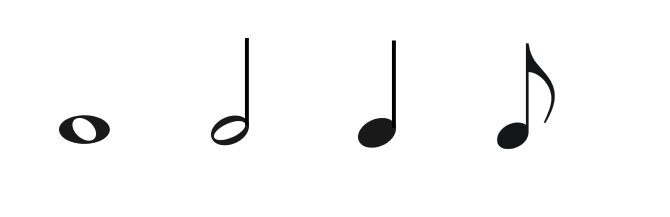
\includegraphics[height=10mm, width=25mm]{
    z_images/3_methodes/0_notation_de_la_batterie/0_figures_de_notes.png}
    \caption{Les figures de notes}
    \label{4_notes}
\end{figure}
La figure \ref{4_notes} montre 4 figures de notes les plus courantes dont les
noms et les durées, exprimées en unité de temps musicale, appelée le «~temps~»
sont respectivement, de gauche à droite~ :
\begin{itemize}
    \item La ronde, elle vaut 4 temps~ ;
    \item La blanche, elle vaut 2 temps~ ;
    \item La noire, elle vaut 1 temps~ ;
    \item La croche, elle vaut 1/2 temps.
\end{itemize}
Une figure de note \cite{danhauser} de musique combine plusieurs éléments
\cite{gould2016behind}
\begin{itemize}
	\item Une tête de note~ :\\
	Sa position sur la portée indique la hauteur de la note. La tête de note
    peut aussi indiquer une durée.
	\item Une hampe~ :\\
	c’est une barre verticale liée à la tête de note. Elle est indicatrice
    d’une durée représentée par sa présence ou non (différence entre la ronde
    et la blanche)
	\item Un crochet~ : La durée d’une note est divisée par deux à chaque
     crochet ajouté à la hampe d’une figure de note.\\
\end{itemize}
\begin{figure}[h]
	\centering
	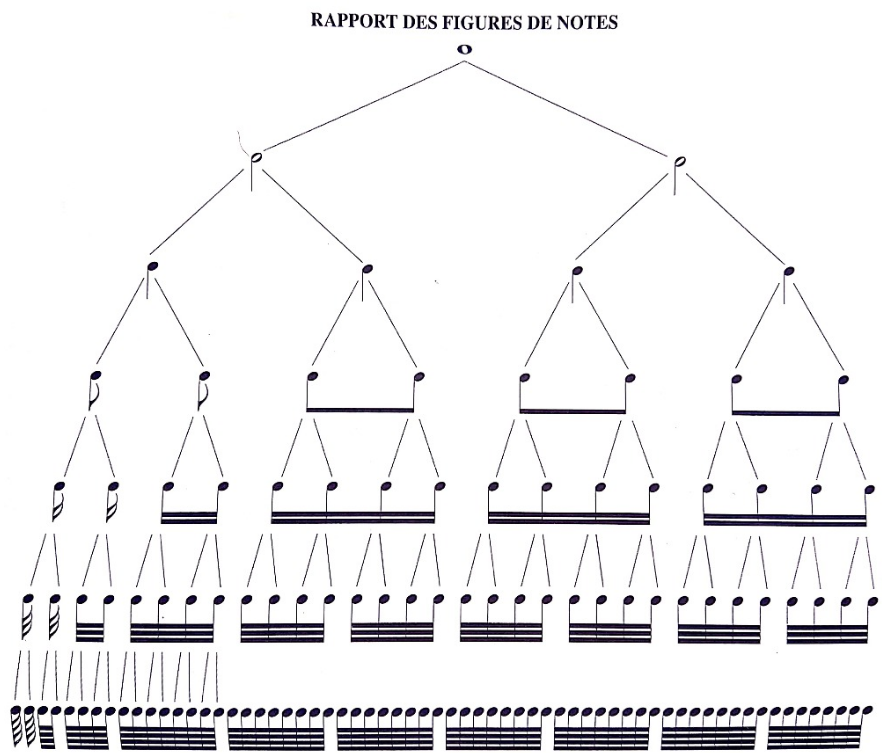
\includegraphics[height=50mm, width=80mm]{
    z_images/3_methodes/0_notation_de_la_batterie/1_rapport_figures_notes.png}
	\caption{Rapport des figures de notes}\cite{danhauser}
	\label{rapp_fig_notes}
\end{figure}

La figure \ref{rapp_fig_notes} montre les rapports de durée entre les figures
de notes. Plus les durées sont longues, plus elles sont marquées par la tête de
note ou la présence ou non de la hampe. À partir de la noire (3ème lignes en
partant du haut), on ajoute un crochet à la hampe d’une figure de notes pour
diviser sa durée par 2. 
Les notes à crochet (croches, doubles-croches, triples-croches,…) 
peuvent être reliées ou non par des ligatures (voir les 4 dernières lignes de
la figure \ref{rapp_fig_notes}).\newpage
\begin{figure}[h]
	\centering
	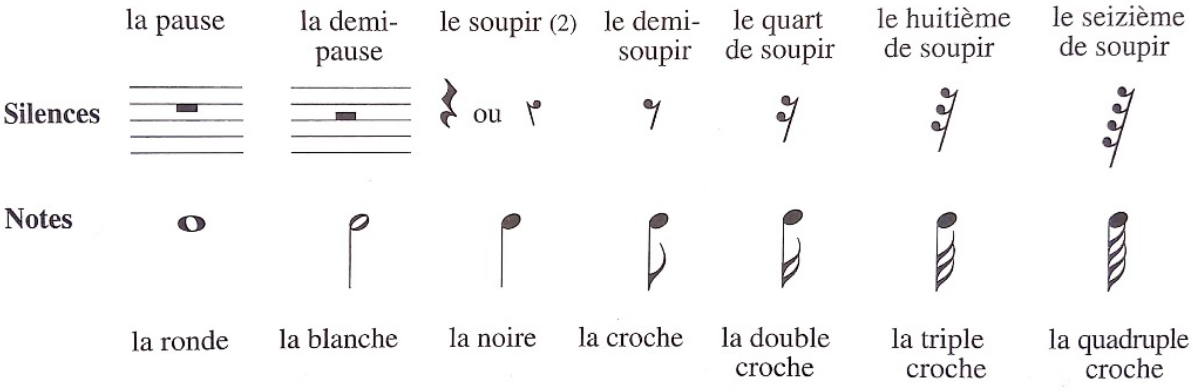
\includegraphics[height=25mm, width=95mm]{
    z_images/3_methodes/0_notation_de_la_batterie/4_silences.png}
	\caption{Les silences}\cite{danhauser}
	\label{silences}
\end{figure}
«~Les silences sont des signes qui indiquent l’interruption du son.~»
\cite{danhauser}. La figure \ref{silences} montre pour chaque figure de note,
la figure de silence qui lui correspond.\\

La transcription sert à traduire les trois caractéristiques du son musical~ :
\begin{itemize}
	\item la hauteur, nombre de vibrations en un temps donné (son grave ou
        aigu — do, ré, mi,…)~ ;
	\item l’intensité, l’amplitude des vibrations (la force du son)~ ;
	\item le timbre, il permet de différencier deux instruments même s’ils
        jouent un son de même hauteur et de même intensité.
\end{itemize}

Ainsi que de leurs combinaisons appelées à former l’ossature de l’œuvre
musicale dans son déroulement temporel, à la fois~ :
\begin{itemize}
	\item diachronique (succession des instants, ce qui constitue en musique la
        mélodie)~ ;
	\item et synchronique (simultanéité des sons, c’est-à-dire l’harmonie).\\
\end{itemize}

Les partitions ont un aspect structuré (hiérarchique). Elles sont divisées en
parties égales que l’on nomme «~mesures~». Les mesures sont séparées par des
barres verticales et sont elles-mêmes divisées implicitement en temps, qui sont
eux-mêmes subdivisés. Le nombre de temps par mesure et le type de leurs
subdivisions par défaut (binaire, ternaire,…) sont déterminés par une fraction
que l’on nomme «~indication de mesure~» ou «~signature rythmique~».\\

\begin{itemize}
    \item $\frac{4}{4}$ $\to$ mesure à 4 temps binaire dont l’unité de temps
        est la noire~ ;\\
    \item $\frac{3}{4}$ $\to$ mesure à 3 temps binaire dont l’unité de temps
        est la noire~ ;\\
    \item $\frac{6}{8}$ $\to$ mesure à 2 temps ternaire dont l’unité de temps
        est la noire pointée \footnote{«~Pointée~» signifie que l’on rajoute à
        la durée d’une note la moitié de sa valeur. Une noire pointée vaut
    trois croches.}.\\
\end{itemize}

La fraction de la signature rythmique est construite par rapport à la ronde.
La fraction 4/4 signifie quatre quarts d’une ronde.\\

Pour les instruments mélodiques, un groupe de notes peut être organisé en
voix, représentant des flots mélodiques joués en parallèle, avec une
synchronisation plus ou moins stricte \cite{shibata} \cite{
Guiomard-Kagan}.

\subsection*{Les données MIDI}
Le format MIDI\footnote{https://www.midi.org/} est originellement une norme
technique mais il peut également être considéré comme une représentation
musicale. Celle-ci peut effectivement être enregistrée par des instruments
compatibles, et visualisée ou jouée par un ordinateur. Ce format historique,
encore très largement utilisé, est très important (mais aussi contraignant)
dans le cadre de notre travail, dans la mesure où de nombreux logiciels
l’utilisent. Pour la transcription musicale, il constitue une strate
intermédiaire très utile entre le signal audio (enregistrement) et la
représentation musicale lisible par un humain (partition).

Il s’agit d’un protocole en temps réel pour échanger des messages et un format
de fichier. Un fichier MIDI est une séquence d’évènements datés et il
représente une performance musicale symbolique.

\begin{figure}[h]
	\centering
	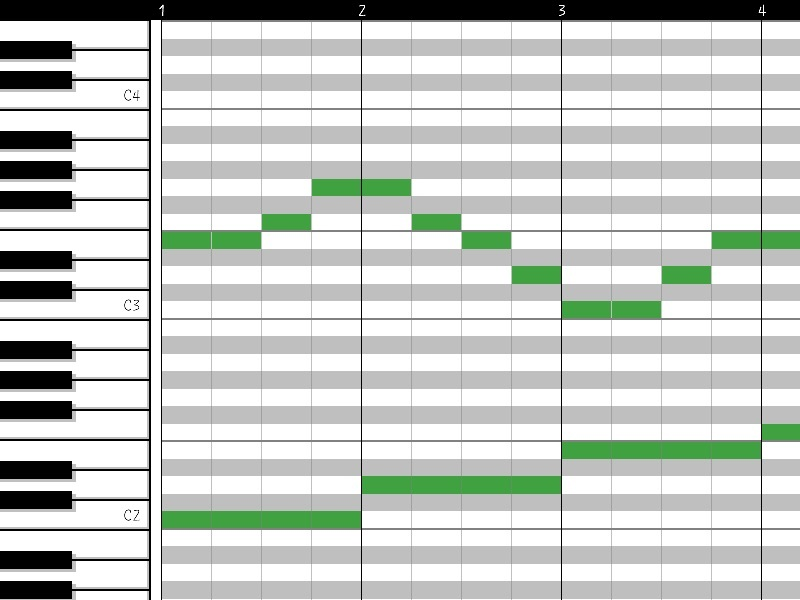
\includegraphics[height=40mm, width=50mm]{
    z_images/1_contexte/2_midi_piano.jpg}
	\caption{Exemple d’évènements MIDI}
	\label{piano_roll}
\end{figure}
Les données MIDI sont représentées sous forme de piano-roll. Chaque bande verte
sur la figure \ref{piano_roll} correspond à une note jouée par un instrument.
Le début (\textit{onset}) et la fin (\textit{offset}) d’une bande verte sont
appelés «~évènement MIDI~». Il existe des évènements ON et des évènements OFF
qui ont chacun une date sur la séquence MIDI. La durée d’une note est
représentée par la distance entre les évènements ON et OFF qui lui
correspondent.\\

Liste des élèments principaux d’un évènement MIDI~ :
\begin{itemize}
    \item type de l’évènement, ON ou OFF~ ;
    \item date de l’évènement, sa position sur la séquence~ ;
    \item pitch de l’évènement, à quelle note il correspond (à quelle
        instrument pour la batterie)~ ;
    \item velocité, volume sonore de l’évènement.\\
\end{itemize}

\subsection*{Les formats XML}
Il existe plusieurs formats XML dédiés à la musique~ : MusicXML, MEI, MNX, …

L’inconvénient de ces formats est qu’ils sont verbeux et ambigus, c’est
pourquoi nous utilisons pour la transcription une représentation intermédiaire
abstraite décrite plus loin.


\begin{figure}[h]
	\centering
	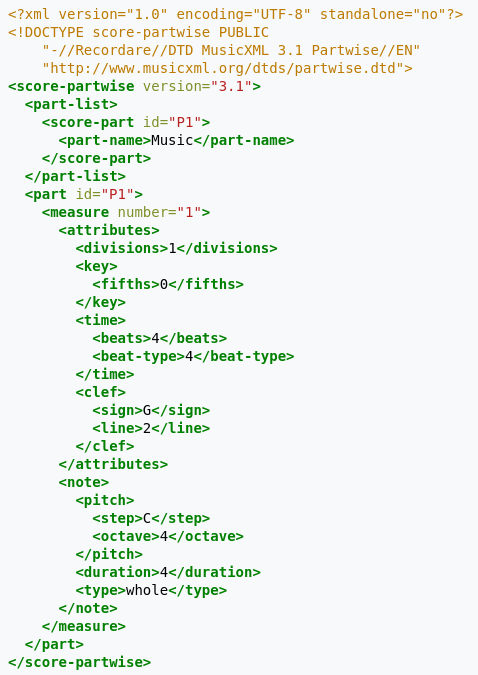
\includegraphics[height=50mm, width=50mm]{
    z_images/1_contexte/6_musicxml_0.png}
    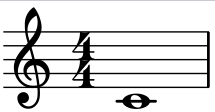
\includegraphics[height=15mm, width=30mm]{
    z_images/1_contexte/6_musicxml_1.png}
	\caption{Exemple de représentation MusicXML} 
	\label{MusicXML}
\end{figure}

Le figure \ref{MusicXML}
\footnote{\textit{Source images~ :
\url{https://fr.wikipedia.org/wiki/MusicXML}}}
représente un do en clef de sol de la durée d’une ronde sur une mesure en 4/4
écrit au format MusicXML.
Un des avantages de ce format est qu’il peut être converti aussi bien en
données MIDI qu’en partition musicale, ce qui en fait un bon format
intermédiaire pour manipuler les données musicales et les échanger entre les
programmes.

\section*{Conclusion}
Dans ce chapitre, nous avons établi que la RIM a connu un fort développement
ces dernières années, et qu’elle s’inspire de plus en plus de méthodes TAL. Par
ce biais, nous avons déduit qu’il existait des liens possibles entre le
traitement du langage musical et celui des langues naturelles, le plus proche
étant probablement le phénomène de transcription (par analogie avec le
\textit{speech to text}). Nous avons contextualisé la transcription de la
musique en générale et plus spécifiquement, de la batterie, en évoquant les
applications possibles dans ses deux domaines. Enfin, nous avons présenté les
représentations de la musique qui concernent directement ce mémoire.
